\documentclass[nooutcomes]{ximera}


\graphicspath{
  {./}
  {1-1QuantitativeReasoning/}
  {1-2RelationsAndGraphs/}
  {1-3ChangingInTandem/}
  {2-1LinearEquations/}
  {2-2LinearModeling/}
  {2-3ExponentialModeling/}
  {3-1WhatIsAFunction/}
  {3-2FunctionProperties/}
  {3-3AverageRatesOfChange/}
  {4-1BuildingNewFunctions/}
  {4-2Polynomials/}
  {5-1RationalFunctions/}
   {5-2ExponentialFunctions/}
  {6-1Domain/}
  {6-2Range/}
  {6-3CompositionOfFunctions/}
  {7-1ZerosOfFunctions/}
  {7-XZerosOfPolynomials/}
  {7-2ZerosOfFamousFunctions/}
  {8-0Review/}
  {8-1FunctionTransformations/}
  {8-2SolvingInequalities/}
  {8-3FunctionTransformationsProject/}
  {9-1RightTriangleTrig/}
  {9-2TheUnitCircle/}
  {9-3TrigIdentities/}
  {10-1UnitCircleToFunctionGraph/}
  {10-2TrigFunctions/}
  {10-3SomeApplicationsOfTrig/}
  {11-1InverseFunctionsRevisited/}
  {11-2Logarithms/}
  {11-3InverseTrig/}
  {12-1SystemsOfEquations/}
  {12-2NonlinearSystems/}
  {12-3ApplicationsOfSystems/}
  {13-1SecantLinesRevisited/}
  {13-2Functions-TheBigPicture/}
  {14-1DisplacementVsDistance/}
  {1-1QuantitativeReasoning/exercises/}
  {1-2RelationsAndGraphs/exercises/}
  {../1-3ChangingInTandem/exercises/}
  {../2-1LinearEquations/exercises/}
  {../2-2LinearModeling/exercises/}
  {../2-3ExponentialModeling/exercises/}
  {../3-1WhatIsAFunction/exercises/}
  {../3-2FunctionProperties/exercises/}
  {../3-3AverageRatesOfChange/exercises/}
  {../5-2ExponentialFunctions/exercises/}
  {../4-1BuildingNewFunctions/exercises/}
  {../4-2Polynomials/exercises/}
  {../5-1RationalFunctions/exercises/}
  {../6-1Domain/exercises/}
  {../6-2Range/exercises/}
  {../6-3CompositionOfFunctions/exercises/}
  {../7-1ZerosOfFunctions/exercises/}
  {../7-XZerosOfPolynomials/exercises/}
  {../7-2ZerosOfFamousFunctions/exercises/}
  {../8-1FunctionTransformations/exercises/}
  {../12-1SystemsOfEquations/exercises/}
  {../8-3FunctionTransformationsProject/exercises/}
  {../8-0Review/exercises/}
  {../8-2SolvingInequalities/exercises/}
  {../8-3FunctionTransformationsProject/exercises/}
  {../9-1RightTriangleTrig/exercises/}
  {../9-2TheUnitCircle/exercises/}
  {../9-3TrigIdentities/exercises/}
  {../10-1UnitCircleToFunctionGraph/exercises/}
  {../10-2TrigFunctions/exercises/}
  {../10-3SomeApplicationsOfTrig/exercises/}
  {../11-1InverseFunctionsRevisited/exercises/}
  {../11-2Logarithms/exercises/}
  {../11-3InverseTrig/exercises/}
  {../12-1SystemsOfEquations/exercises/}
  {../12-2NonlinearSystems/exercises/}
  {../12-3ApplicationsOfSystems/exercises/}
  {../13-1SecantLinesRevisited/exercises/}
  {../13-2Functions-TheBigPicture/exercises/}
  {../14-1DisplacementVsDistance/exercises/}
}

\DeclareGraphicsExtensions{.pdf,.png,.jpg,.eps}

\newcommand{\mooculus}{\textsf{\textbf{MOOC}\textnormal{\textsf{ULUS}}}}

\usepackage[makeroom]{cancel} %% for strike outs

\ifxake
\else
\usepackage[most]{tcolorbox}
\fi


%\typeout{************************************************}
%\typeout{New Environments}
%\typeout{************************************************}

%% to fix for web can be removed when deployed offically with ximera2
\let\image\relax\let\endimage\relax
\NewEnviron{image}{% 
  \begin{center}\BODY\end{center}% center
}



\NewEnviron{folder}{
      \addcontentsline{toc}{section}{\textbf{\BODY}}
}

\ifxake
\let\summary\relax
\let\endsummary\relax
\newtheorem*{summary}{Summary}
\newtheorem*{callout}{Callout}
\newtheorem*{overview}{Overview}
\newtheorem*{objectives}{Objectives}
\newtheorem*{motivatingQuestions}{Motivating Questions}
\newtheorem*{MM}{Metacognitive Moment}
      
%% NEEDED FOR XIMERA 2
%\ximerizedEnvironment{summary}
%\ximerizedEnvironment{callout}
%\ximerizedEnvironment{overview} 
%\ximerizedEnvironment{objectives}
%\ximerizedEnvironment{motivatingQuestions}
%\ximerizedEnvironment{MM}
\else
%% CALLOUT
\NewEnviron{callout}{
  \begin{tcolorbox}[colback=blue!5, breakable,pad at break*=1mm]
      \BODY
  \end{tcolorbox}
}
%% MOTIVATING QUESTIONS
\NewEnviron{motivatingQuestions}{
  \begin{tcolorbox}[ breakable,pad at break*=1mm]
    \textbf{\Large Motivating Questions}\hfill
    %\begin{itemize}[label=\textbullet]
      \BODY
    %\end{itemize}
  \end{tcolorbox}
}
%% OBJECTIVES
\NewEnviron{objectives}{  
    \vspace{.5in}
      %\begin{tcolorbox}[colback=orange!5, breakable,pad at break*=1mm]
    \textbf{\Large Learning Objectives}
    \begin{itemize}[label=\textbullet]
      \BODY
    \end{itemize}
    %\end{tcolorbox}
}
%% DEFINITION
\let\definition\relax
\let\enddefinition\relax
\NewEnviron{definition}{
  \begin{tcolorbox}[ breakable,pad at break*=1mm]
    \noindent\textbf{Definition}~
      \BODY
  \end{tcolorbox}
}
%% OVERVIEW
\let\overview\relax
\let\overview\relax
\NewEnviron{overview}{
  \begin{tcolorbox}[ breakable,pad at break*=1mm]
    \textbf{\Large Overview}
    %\begin{itemize}[label=\textbullet] %% breaks Xake
      \BODY
    %\end{itemize}
  \end{tcolorbox}
}
%% SUMMARY
\let\summary\relax
\let\endsummary\relax
\NewEnviron{summary}{
  \begin{tcolorbox}[ breakable,pad at break*=1mm]
    \textbf{\Large Summary}
    %\begin{itemize}[label=\textbullet] %% breaks Xake
      \BODY
    %\end{itemize}
  \end{tcolorbox}
}
%% REMARK
\let\remark\relax
\let\endremark\relax
\NewEnviron{remark}{
  \begin{tcolorbox}[colback=green!5, breakable,pad at break*=1mm]
    \noindent\textbf{Remark}~
      \BODY
  \end{tcolorbox}
}
%% EXPLANATION
\let\explanation\relax
\let\endexplanation\relax
\NewEnviron{explanation}{
    \normalfont
    \noindent\textbf{Explanation}~
      \BODY
}
%% EXPLORATION
\let\exploration\relax
\let\endexploration\relax
\NewEnviron{exploration}{
  \begin{tcolorbox}[colback=yellow!10, breakable,pad at break*=1mm]
    \noindent\textbf{Exploration}~
      \BODY
  \end{tcolorbox}
}
%% METACOGNITIVE MOMENTS
\let\MM\relax
\let\endMM\relax
\NewEnviron{MM}{
  \begin{tcolorbox}[colback=pink!15, breakable,pad at break*=1mm]
    \noindent\textbf{Metacognitive Moment}~
      \BODY
  \end{tcolorbox}
}


\fi





%Notes on what envirnoment to use:  Example with Explanation in text; if they are supposed to answer- Problem; no answer - Exploration


%\typeout{************************************************}
%% Header and footers
%\typeout{************************************************}

\newcommand{\licenseAcknowledgement}{Licensed under Creative Commons 4.0}
\newcommand{\licenseAPC}{\renewcommand{\licenseAcknowledgement}{\textbf{Acknowledgements:} Active Prelude to Calculus (https://activecalculus.org/prelude) }}
\newcommand{\licenseSZ}{\renewcommand{\licenseAcknowledgement}{\textbf{Acknowledgements:} Stitz Zeager Open Source Mathematics (https://www.stitz-zeager.com/) }}
\newcommand{\licenseAPCSZ}{\renewcommand{\licenseAcknowledgement}{\textbf{Acknowledgements:} Active Prelude to Calculus (https://activecalculus.org/prelude) and Stitz Zeager Open Source Mathematics (https://www.stitz-zeager.com/) }}
\newcommand{\licenseORCCA}{\renewcommand{\licenseAcknowledgement}{\textbf{Acknowledgements:}Original source material, products with readable and accessible
math content, and other information freely available at pcc.edu/orcca.}}
\newcommand{\licenseY}{\renewcommand{\licenseAcknowledgement}{\textbf{Acknowledgements:} Yoshiwara Books (https://yoshiwarabooks.org/)}}
\newcommand{\licenseOS}{\renewcommand{\licenseAcknowledgement}{\textbf{Acknowledgements:} OpenStax College Algebra (https://openstax.org/details/books/college-algebra)}}
\newcommand{\licenseAPCSZCSCC}{\renewcommand{\licenseAcknowledgement}{\textbf{Acknowledgements:} Active Prelude to Calculus (https://activecalculus.org/prelude), Stitz Zeager Open Source Mathematics (https://www.stitz-zeager.com/), CSCC PreCalculus and Calculus texts (https://ximera.osu.edu/csccmathematics)}}

\ifxake\else %% do nothing on the website
\usepackage{fancyhdr}
\pagestyle{fancy}
\fancyhf{}
\fancyhead[R]{\sectionmark}
\fancyfoot[L]{\thepage}
\fancyfoot[C]{\licenseAcknowledgement}
\renewcommand{\headrulewidth}{0pt}
\renewcommand{\footrulewidth}{0pt}
\fi

%%%%%%%%%%%%%%%%



%\typeout{************************************************}
%\typeout{Table of Contents}
%\typeout{************************************************}


%% Edit this to change the font style
\newcommand{\sectionHeadStyle}{\sffamily\bfseries}


\makeatletter

%% part uses arabic numerals
\renewcommand*\thepart{\arabic{part}}


\ifxake\else
\renewcommand\chapterstyle{%
  \def\maketitle{%
    \addtocounter{titlenumber}{1}%
    \pagestyle{fancy}
    \phantomsection
    \addcontentsline{toc}{section}{\textbf{\thepart.\thetitlenumber\hspace{1em}\@title}}%
                    {\flushleft\small\sectionHeadStyle\@pretitle\par\vspace{-1.5em}}%
                    {\flushleft\LARGE\sectionHeadStyle\thepart.\thetitlenumber\hspace{1em}\@title \par }%
                    {\setcounter{problem}{0}\setcounter{sectiontitlenumber}{0}}%
                    \par}}





\renewcommand\sectionstyle{%
  \def\maketitle{%
    \addtocounter{sectiontitlenumber}{1}
    \pagestyle{fancy}
    \phantomsection
    \addcontentsline{toc}{subsection}{\thepart.\thetitlenumber.\thesectiontitlenumber\hspace{1em}\@title}%
    {\flushleft\small\sectionHeadStyle\@pretitle\par\vspace{-1.5em}}%
    {\flushleft\Large\sectionHeadStyle\thepart.\thetitlenumber.\thesectiontitlenumber\hspace{1em}\@title \par}%
    %{\setcounter{subsectiontitlenumber}{0}}%
    \par}}



\renewcommand\section{\@startsection{paragraph}{10}{\z@}%
                                     {-3.25ex\@plus -1ex \@minus -.2ex}%
                                     {1.5ex \@plus .2ex}%
                                     {\normalfont\large\sectionHeadStyle}}
\renewcommand\subsection{\@startsection{subparagraph}{10}{\z@}%
                                    {3.25ex \@plus1ex \@minus.2ex}%
                                    {-1em}%
                                    {\normalfont\normalsize\sectionHeadStyle}}

\fi

%% redefine Part
\renewcommand\part{%
   {\setcounter{titlenumber}{0}}
  \if@openright
    \cleardoublepage
  \else
    \clearpage
  \fi
  \thispagestyle{plain}%
  \if@twocolumn
    \onecolumn
    \@tempswatrue
  \else
    \@tempswafalse
  \fi
  \null\vfil
  \secdef\@part\@spart}

\def\@part[#1]#2{%
    \ifnum \c@secnumdepth >-2\relax
      \refstepcounter{part}%
      \addcontentsline{toc}{part}{\thepart\hspace{1em}#1}%
    \else
      \addcontentsline{toc}{part}{#1}%
    \fi
    \markboth{}{}%
    {\centering
     \interlinepenalty \@M
     \normalfont
     \ifnum \c@secnumdepth >-2\relax
       \huge\sffamily\bfseries \partname\nobreakspace\thepart
       \par
       \vskip 20\p@
     \fi
     \Huge \bfseries #2\par}%
    \@endpart}
\def\@spart#1{%
    {\centering
     \interlinepenalty \@M
     \normalfont
     \Huge \bfseries #1\par}%
    \@endpart}
\def\@endpart{\vfil\newpage
              \if@twoside
               \if@openright
                \null
                \thispagestyle{empty}%
                \newpage
               \fi
              \fi
              \if@tempswa
                \twocolumn
                \fi}



\makeatother





%\typeout{************************************************}
%\typeout{Stuff from Ximera}
%\typeout{************************************************}



\usepackage{array}  %% This is for typesetting long division
\setlength{\extrarowheight}{+.1cm}
\newdimen\digitwidth
\settowidth\digitwidth{9}
\def\divrule#1#2{
\noalign{\moveright#1\digitwidth
\vbox{\hrule width#2\digitwidth}}}





\newcommand{\RR}{\mathbb R}
\newcommand{\R}{\mathbb R}
\newcommand{\N}{\mathbb N}
\newcommand{\Z}{\mathbb Z}

\newcommand{\sagemath}{\textsf{SageMath}}


\def\d{\,d}
%\renewcommand{\d}{\mathop{}\!d}
\newcommand{\dd}[2][]{\frac{\d #1}{\d #2}}
\newcommand{\pp}[2][]{\frac{\partial #1}{\partial #2}}
\renewcommand{\l}{\ell}
\newcommand{\ddx}{\frac{d}{\d x}}



%\newcommand{\unit}{\,\mathrm}
\newcommand{\unit}{\mathop{}\!\mathrm}
\newcommand{\eval}[1]{\bigg[ #1 \bigg]}
\newcommand{\seq}[1]{\left( #1 \right)}
\renewcommand{\epsilon}{\varepsilon}
\renewcommand{\phi}{\varphi}


\renewcommand{\iff}{\Leftrightarrow}

\DeclareMathOperator{\arccot}{arccot}
\DeclareMathOperator{\arcsec}{arcsec}
\DeclareMathOperator{\arccsc}{arccsc}
\DeclareMathOperator{\sign}{sign}


%\DeclareMathOperator{\divergence}{divergence}
%\DeclareMathOperator{\curl}[1]{\grad\cross #1}
\newcommand{\lto}{\mathop{\longrightarrow\,}\limits}

\renewcommand{\bar}{\overline}

\colorlet{textColor}{black}
\colorlet{background}{white}
\colorlet{penColor}{blue!50!black} % Color of a curve in a plot
\colorlet{penColor2}{red!50!black}% Color of a curve in a plot
\colorlet{penColor3}{red!50!blue} % Color of a curve in a plot
\colorlet{penColor4}{green!50!black} % Color of a curve in a plot
\colorlet{penColor5}{orange!80!black} % Color of a curve in a plot
\colorlet{penColor6}{yellow!70!black} % Color of a curve in a plot
\colorlet{fill1}{penColor!20} % Color of fill in a plot
\colorlet{fill2}{penColor2!20} % Color of fill in a plot
\colorlet{fillp}{fill1} % Color of positive area
\colorlet{filln}{penColor2!20} % Color of negative area
\colorlet{fill3}{penColor3!20} % Fill
\colorlet{fill4}{penColor4!20} % Fill
\colorlet{fill5}{penColor5!20} % Fill
\colorlet{gridColor}{gray!50} % Color of grid in a plot

\newcommand{\surfaceColor}{violet}
\newcommand{\surfaceColorTwo}{redyellow}
\newcommand{\sliceColor}{greenyellow}




\pgfmathdeclarefunction{gauss}{2}{% gives gaussian
  \pgfmathparse{1/(#2*sqrt(2*pi))*exp(-((x-#1)^2)/(2*#2^2))}%
}





%\typeout{************************************************}
%\typeout{ORCCA Preamble.Tex}
%\typeout{************************************************}


%% \usepackage{geometry}
%% \geometry{letterpaper,total={408pt,9.0in}}
%% Custom Page Layout Adjustments (use latex.geometry)
%% \usepackage{amsmath,amssymb}
%% \usepackage{pgfplots}
\usepackage{pifont}                                         %needed for symbols, s.a. airplane symbol
\usetikzlibrary{positioning,fit,backgrounds}                %needed for nested diagrams
\usetikzlibrary{calc,trees,positioning,arrows,fit,shapes}   %needed for set diagrams
\usetikzlibrary{decorations.text}                           %needed for text following a curve
\usetikzlibrary{arrows,arrows.meta}                         %needed for open/closed intervals
\usetikzlibrary{positioning,3d,shapes.geometric}            %needed for 3d number sets tower

%% NEEDED FOR XIMERA 1
%\usetkzobj{all}       %NO LONGER VALID
%%%%%%%%%%%%%%

\usepackage{tikz-3dplot}
\usepackage{tkz-euclide}                     %needed for triangle diagrams
\usepgfplotslibrary{fillbetween}                            %shade regions of a plot
\usetikzlibrary{shadows}                                    %function diagrams
\usetikzlibrary{positioning}                                %function diagrams
\usetikzlibrary{shapes}                                     %function diagrams
%%% global colors from https://www.pcc.edu/web-services/style-guide/basics/color/ %%%
\definecolor{ruby}{HTML}{9E0C0F}
\definecolor{turquoise}{HTML}{008099}
\definecolor{emerald}{HTML}{1c8464}
\definecolor{amber}{HTML}{c7502a}
\definecolor{amethyst}{HTML}{70485b}
\definecolor{sapphire}{HTML}{263c53}
\colorlet{firstcolor}{sapphire}
\colorlet{secondcolor}{turquoise}
\colorlet{thirdcolor}{emerald}
\colorlet{fourthcolor}{amber}
\colorlet{fifthcolor}{amethyst}
\colorlet{sixthcolor}{ruby}
\colorlet{highlightcolor}{green!50!black}
\colorlet{graphbackground}{white}
\colorlet{wood}{brown!60!white}
%%% curve, dot, and graph custom styles %%%
\pgfplotsset{firstcurve/.style      = {color=firstcolor,  mark=none, line width=1pt, {Kite}-{Kite}, solid}}
\pgfplotsset{secondcurve/.style     = {color=secondcolor, mark=none, line width=1pt, {Kite}-{Kite}, solid}}
\pgfplotsset{thirdcurve/.style      = {color=thirdcolor,  mark=none, line width=1pt, {Kite}-{Kite}, solid}}
\pgfplotsset{fourthcurve/.style     = {color=fourthcolor, mark=none, line width=1pt, {Kite}-{Kite}, solid}}
\pgfplotsset{fifthcurve/.style      = {color=fifthcolor,  mark=none, line width=1pt, {Kite}-{Kite}, solid}}
\pgfplotsset{highlightcurve/.style  = {color=highlightcolor,  mark=none, line width=5pt, -, opacity=0.3}}   % thick, opaque curve for highlighting
\pgfplotsset{asymptote/.style       = {color=gray, mark=none, line width=1pt, <->, dashed}}
\pgfplotsset{symmetryaxis/.style    = {color=gray, mark=none, line width=1pt, <->, dashed}}
\pgfplotsset{guideline/.style       = {color=gray, mark=none, line width=1pt, -}}
\tikzset{guideline/.style           = {color=gray, mark=none, line width=1pt, -}}
\pgfplotsset{altitude/.style        = {dashed, color=gray, thick, mark=none, -}}
\tikzset{altitude/.style            = {dashed, color=gray, thick, mark=none, -}}
\pgfplotsset{radius/.style          = {dashed, thick, mark=none, -}}
\tikzset{radius/.style              = {dashed, thick, mark=none, -}}
\pgfplotsset{rightangle/.style      = {color=gray, mark=none, -}}
\tikzset{rightangle/.style          = {color=gray, mark=none, -}}
\pgfplotsset{closedboundary/.style  = {color=black, mark=none, line width=1pt, {Kite}-{Kite},solid}}
\tikzset{closedboundary/.style      = {color=black, mark=none, line width=1pt, {Kite}-{Kite},solid}}
\pgfplotsset{openboundary/.style    = {color=black, mark=none, line width=1pt, {Kite}-{Kite},dashed}}
\tikzset{openboundary/.style        = {color=black, mark=none, line width=1pt, {Kite}-{Kite},dashed}}
\tikzset{verticallinetest/.style    = {color=gray, mark=none, line width=1pt, <->,dashed}}
\pgfplotsset{soliddot/.style        = {color=firstcolor,  mark=*, only marks}}
\pgfplotsset{hollowdot/.style       = {color=firstcolor,  mark=*, only marks, fill=graphbackground}}
\pgfplotsset{blankgraph/.style      = {xmin=-10, xmax=10,
                                        ymin=-10, ymax=10,
                                        axis line style={-, draw opacity=0 },
                                        axis lines=box,
                                        major tick length=0mm,
                                        xtick={-10,-9,...,10},
                                        ytick={-10,-9,...,10},
                                        grid=major,
                                        grid style={solid,gray!20},
                                        xticklabels={,,},
                                        yticklabels={,,},
                                        minor xtick=,
                                        minor ytick=,
                                        xlabel={},ylabel={},
                                        width=0.75\textwidth,
                                      }
            }
\pgfplotsset{numberline/.style      = {xmin=-10,xmax=10,
                                        minor xtick={-11,-10,...,11},
                                        xtick={-10,-5,...,10},
                                        every tick/.append style={thick},
                                        axis y line=none,
                                        y=15pt,
                                        axis lines=middle,
                                        enlarge x limits,
                                        grid=none,
                                        clip=false,
                                        axis background/.style={},
                                        after end axis/.code={
                                          \path (axis cs:0,0)
                                          node [anchor=north,yshift=-0.075cm] {\footnotesize 0};
                                        },
                                        every axis x label/.style={at={(current axis.right of origin)},anchor=north},
                                      }
            }
\pgfplotsset{openinterval/.style={color=firstcolor,mark=none,ultra thick,{Parenthesis}-{Parenthesis}}}
\pgfplotsset{openclosedinterval/.style={color=firstcolor,mark=none,ultra thick,{Parenthesis}-{Bracket}}}
\pgfplotsset{closedinterval/.style={color=firstcolor,mark=none,ultra thick,{Bracket}-{Bracket}}}
\pgfplotsset{closedopeninterval/.style={color=firstcolor,mark=none,ultra thick,{Bracket}-{Parenthesis}}}
\pgfplotsset{infiniteopeninterval/.style={color=firstcolor,mark=none,ultra thick,{Kite}-{Parenthesis}}}
\pgfplotsset{openinfiniteinterval/.style={color=firstcolor,mark=none,ultra thick,{Parenthesis}-{Kite}}}
\pgfplotsset{infiniteclosedinterval/.style={color=firstcolor,mark=none,ultra thick,{Kite}-{Bracket}}}
\pgfplotsset{closedinfiniteinterval/.style={color=firstcolor,mark=none,ultra thick,{Bracket}-{Kite}}}
\pgfplotsset{infiniteinterval/.style={color=firstcolor,mark=none,ultra thick,{Kite}-{Kite}}}
\pgfplotsset{interval/.style= {ultra thick, -}}
%%% cycle list of plot styles for graphs with multiple plots %%%
\pgfplotscreateplotcyclelist{pccstylelist}{%
  firstcurve\\%
  secondcurve\\%
  thirdcurve\\%
  fourthcurve\\%
  fifthcurve\\%
}
%%% default plot settings %%%
\pgfplotsset{every axis/.append style={
  axis x line=middle,    % put the x axis in the middle
  axis y line=middle,    % put the y axis in the middle
  axis line style={<->}, % arrows on the axis
  scaled ticks=false,
  tick label style={/pgf/number format/fixed},
  xlabel={$x$},          % default put x on x-axis
  ylabel={$y$},          % default put y on y-axis
  xmin = -7,xmax = 7,    % most graphs have this window
  ymin = -7,ymax = 7,    % most graphs have this window
  domain = -7:7,
  xtick = {-6,-4,...,6}, % label these ticks
  ytick = {-6,-4,...,6}, % label these ticks
  yticklabel style={inner sep=0.333ex},
  minor xtick = {-7,-6,...,7}, % include these ticks, some without label
  minor ytick = {-7,-6,...,7}, % include these ticks, some without label
  scale only axis,       % don't consider axis and tick labels for width and height calculation
  cycle list name=pccstylelist,
  tick label style={font=\footnotesize},
  legend cell align=left,
  grid = both,
  grid style = {solid,gray!20},
  axis background/.style={fill=graphbackground},
}}
\pgfplotsset{framed/.style={axis background/.style ={draw=gray}}}
%\pgfplotsset{framed/.style={axis background/.style ={draw=gray,fill=graphbackground,rounded corners=3ex}}}
%%% other tikz (not pgfplots) settings %%%
%\tikzset{axisnode/.style={font=\scriptsize,text=black}}
\tikzset{>=stealth}
%%% for nested diagram in types of numbers section %%%
\newcommand\drawnestedsets[4]{
  \def\position{#1}             % initial position
  \def\nbsets{#2}               % number of sets
  \def\listofnestedsets{#3}     % list of sets
  \def\reversedlistofcolors{#4} % reversed list of colors
  % position and draw labels of sets
  \coordinate (circle-0) at (#1);
  \coordinate (set-0) at (#1);
  \foreach \set [count=\c] in \listofnestedsets {
    \pgfmathtruncatemacro{\cminusone}{\c - 1}
    % label of current set (below previous nested set)
    \node[below=3pt of circle-\cminusone,inner sep=0]
    (set-\c) {\set};
    % current set (fit current label and previous set)
    \node[circle,inner sep=0,fit=(circle-\cminusone)(set-\c)]
    (circle-\c) {};
  }
  % draw and fill sets in reverse order
  \begin{scope}[on background layer]
    \foreach \col[count=\c] in \reversedlistofcolors {
      \pgfmathtruncatemacro{\invc}{\nbsets-\c}
      \pgfmathtruncatemacro{\invcplusone}{\invc+1}
      \node[circle,draw,fill=\col,inner sep=0,
      fit=(circle-\invc)(set-\invcplusone)] {};
    }
  \end{scope}
  }
\ifdefined\tikzset
\tikzset{ampersand replacement = \amp}
\fi
\newcommand{\abs}[1]{\left\lvert#1\right\rvert}
%\newcommand{\point}[2]{\left(#1,#2\right)}
\newcommand{\highlight}[1]{\definecolor{sapphire}{RGB}{59,90,125} {\color{sapphire}{{#1}}}}
\newcommand{\firsthighlight}[1]{\definecolor{sapphire}{RGB}{59,90,125} {\color{sapphire}{{#1}}}}
\newcommand{\secondhighlight}[1]{\definecolor{emerald}{RGB}{20,97,75} {\color{emerald}{{#1}}}}
\newcommand{\unhighlight}[1]{{\color{black}{{#1}}}}
\newcommand{\lowlight}[1]{{\color{lightgray}{#1}}}
\newcommand{\attention}[1]{\mathord{\overset{\downarrow}{#1}}}
\newcommand{\nextoperation}[1]{\mathord{\boxed{#1}}}
\newcommand{\substitute}[1]{{\color{blue}{{#1}}}}
\newcommand{\pinover}[2]{\overset{\overset{\mathrm{\ #2\ }}{|}}{\strut #1 \strut}}
\newcommand{\addright}[1]{{\color{blue}{{{}+#1}}}}
\newcommand{\addleft}[1]{{\color{blue}{{#1+{}}}}}
\newcommand{\subtractright}[1]{{\color{blue}{{{}-#1}}}}
\newcommand{\multiplyright}[2][\cdot]{{\color{blue}{{{}#1#2}}}}
\newcommand{\multiplyleft}[2][\cdot]{{\color{blue}{{#2#1{}}}}}
\newcommand{\divideunder}[2]{\frac{#1}{{\color{blue}{{#2}}}}}
\newcommand{\divideright}[1]{{\color{blue}{{{}\div#1}}}}
\newcommand{\negate}[1]{{\color{blue}{{-}}}\left(#1\right)}
\newcommand{\cancelhighlight}[1]{\definecolor{sapphire}{RGB}{59,90,125}{\color{sapphire}{{\cancel{#1}}}}}
\newcommand{\secondcancelhighlight}[1]{\definecolor{emerald}{RGB}{20,97,75}{\color{emerald}{{\bcancel{#1}}}}}
\newcommand{\thirdcancelhighlight}[1]{\definecolor{amethyst}{HTML}{70485b}{\color{amethyst}{{\xcancel{#1}}}}}
\newcommand{\lt}{<} %% Bart: WHY?
\newcommand{\gt}{>} %% Bart: WHY?
\newcommand{\amp}{&} %% Bart: WHY?


%%% These commands break Xake
%% \newcommand{\apple}{\text{🍎}}
%% \newcommand{\banana}{\text{🍌}}
%% \newcommand{\pear}{\text{🍐}}
%% \newcommand{\cat}{\text{🐱}}
%% \newcommand{\dog}{\text{🐶}}

\newcommand{\apple}{PICTURE OF APPLE}
\newcommand{\banana}{PICTURE OF BANANA}
\newcommand{\pear}{PICTURE OF PEAR}
\newcommand{\cat}{PICTURE OF CAT}
\newcommand{\dog}{PICTURE OF DOG}


%%%%% INDEX STUFF
\newcommand{\dfn}[1]{\textbf{#1}\index{#1}}
\usepackage{imakeidx}
\makeindex[intoc]
\makeatletter
\gdef\ttl@savemark{\sectionmark{}}
\makeatother












 % for drawing cube in Optimization problem
\usetikzlibrary{quotes,arrows.meta}
\tikzset{
  annotated cuboid/.pic={
    \tikzset{%
      every edge quotes/.append style={midway, auto},
      /cuboid/.cd,
      #1
    }
    \draw [every edge/.append style={pic actions, densely dashed, opacity=.5}, pic actions]
    (0,0,0) coordinate (o) -- ++(-\cubescale*\cubex,0,0) coordinate (a) -- ++(0,-\cubescale*\cubey,0) coordinate (b) edge coordinate [pos=1] (g) ++(0,0,-\cubescale*\cubez)  -- ++(\cubescale*\cubex,0,0) coordinate (c) -- cycle
    (o) -- ++(0,0,-\cubescale*\cubez) coordinate (d) -- ++(0,-\cubescale*\cubey,0) coordinate (e) edge (g) -- (c) -- cycle
    (o) -- (a) -- ++(0,0,-\cubescale*\cubez) coordinate (f) edge (g) -- (d) -- cycle;
    \path [every edge/.append style={pic actions, |-|}]
    (b) +(0,-5pt) coordinate (b1) edge ["x"'] (b1 -| c)
    (b) +(-5pt,0) coordinate (b2) edge ["y"] (b2 |- a)
    (c) +(3.5pt,-3.5pt) coordinate (c2) edge ["x"'] ([xshift=3.5pt,yshift=-3.5pt]e)
    ;
  },
  /cuboid/.search also={/tikz},
  /cuboid/.cd,
  width/.store in=\cubex,
  height/.store in=\cubey,
  depth/.store in=\cubez,
  units/.store in=\cubeunits,
  scale/.store in=\cubescale,
  width=10,
  height=10,
  depth=10,
  units=cm,
  scale=.1,
}

\author{Elizabeth Miller}
\license{Creative Commons Attribution-ShareAlike 4.0 International License}
\acknowledgement{https://activecalculus.org/}

\title{The Sine and Cosine Functions}

\begin{document}
\licenseAPC
\begin{abstract}
  
\end{abstract}
\maketitle


%\typeout{************************************************}
%\typeout{Motivating Questions}
%\typeout{************************************************}

\begin{motivatingQuestions}\begin{itemize}
\item What are the sine and cosine functions and how do they arise from a point traversing the unit circle?%
\item What important properties do the sine and cosine functions share?%
\end{itemize}\end{motivatingQuestions}


%\typeout{************************************************}
%\typeout{Introduction}
%\typeout{************************************************}

In the last section, we saw how tracking the height of a point that is traversing a circle generates a periodic function.  Previously, we also identified a collection of special points on the unit circle.
\begin{image}
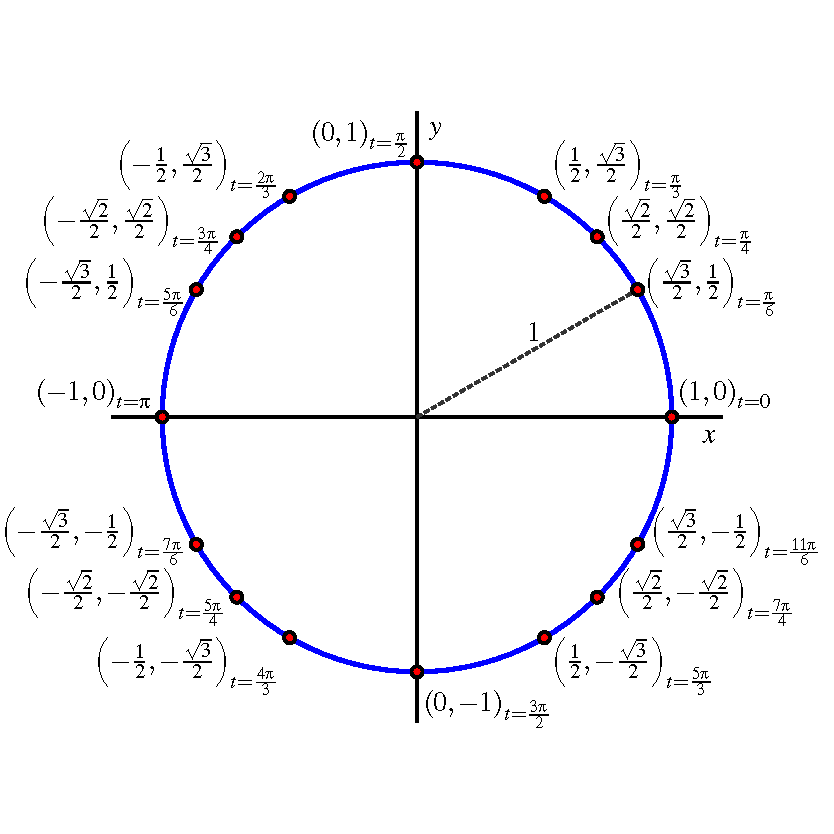
\includegraphics[width=\textwidth]{unit-circle-16-all-labeled.png}
\end{image}

You can also use the \emph{Desmos} file:

\begin{center}  
\desmos{jgddn7tzxg}{800}{600}  
\end{center}

\begin{exploration}

If we consider the unit circle, start at \(t = 0\), and traverse the circle counterclockwise, we may view the height, \(h\), of the traversing point as a function of the angle, \(t\), in radians.  From there, we can plot the resulting \((t,h)\) ordered pairs and connect them to generate the circular function pictured below.

\begin{image}
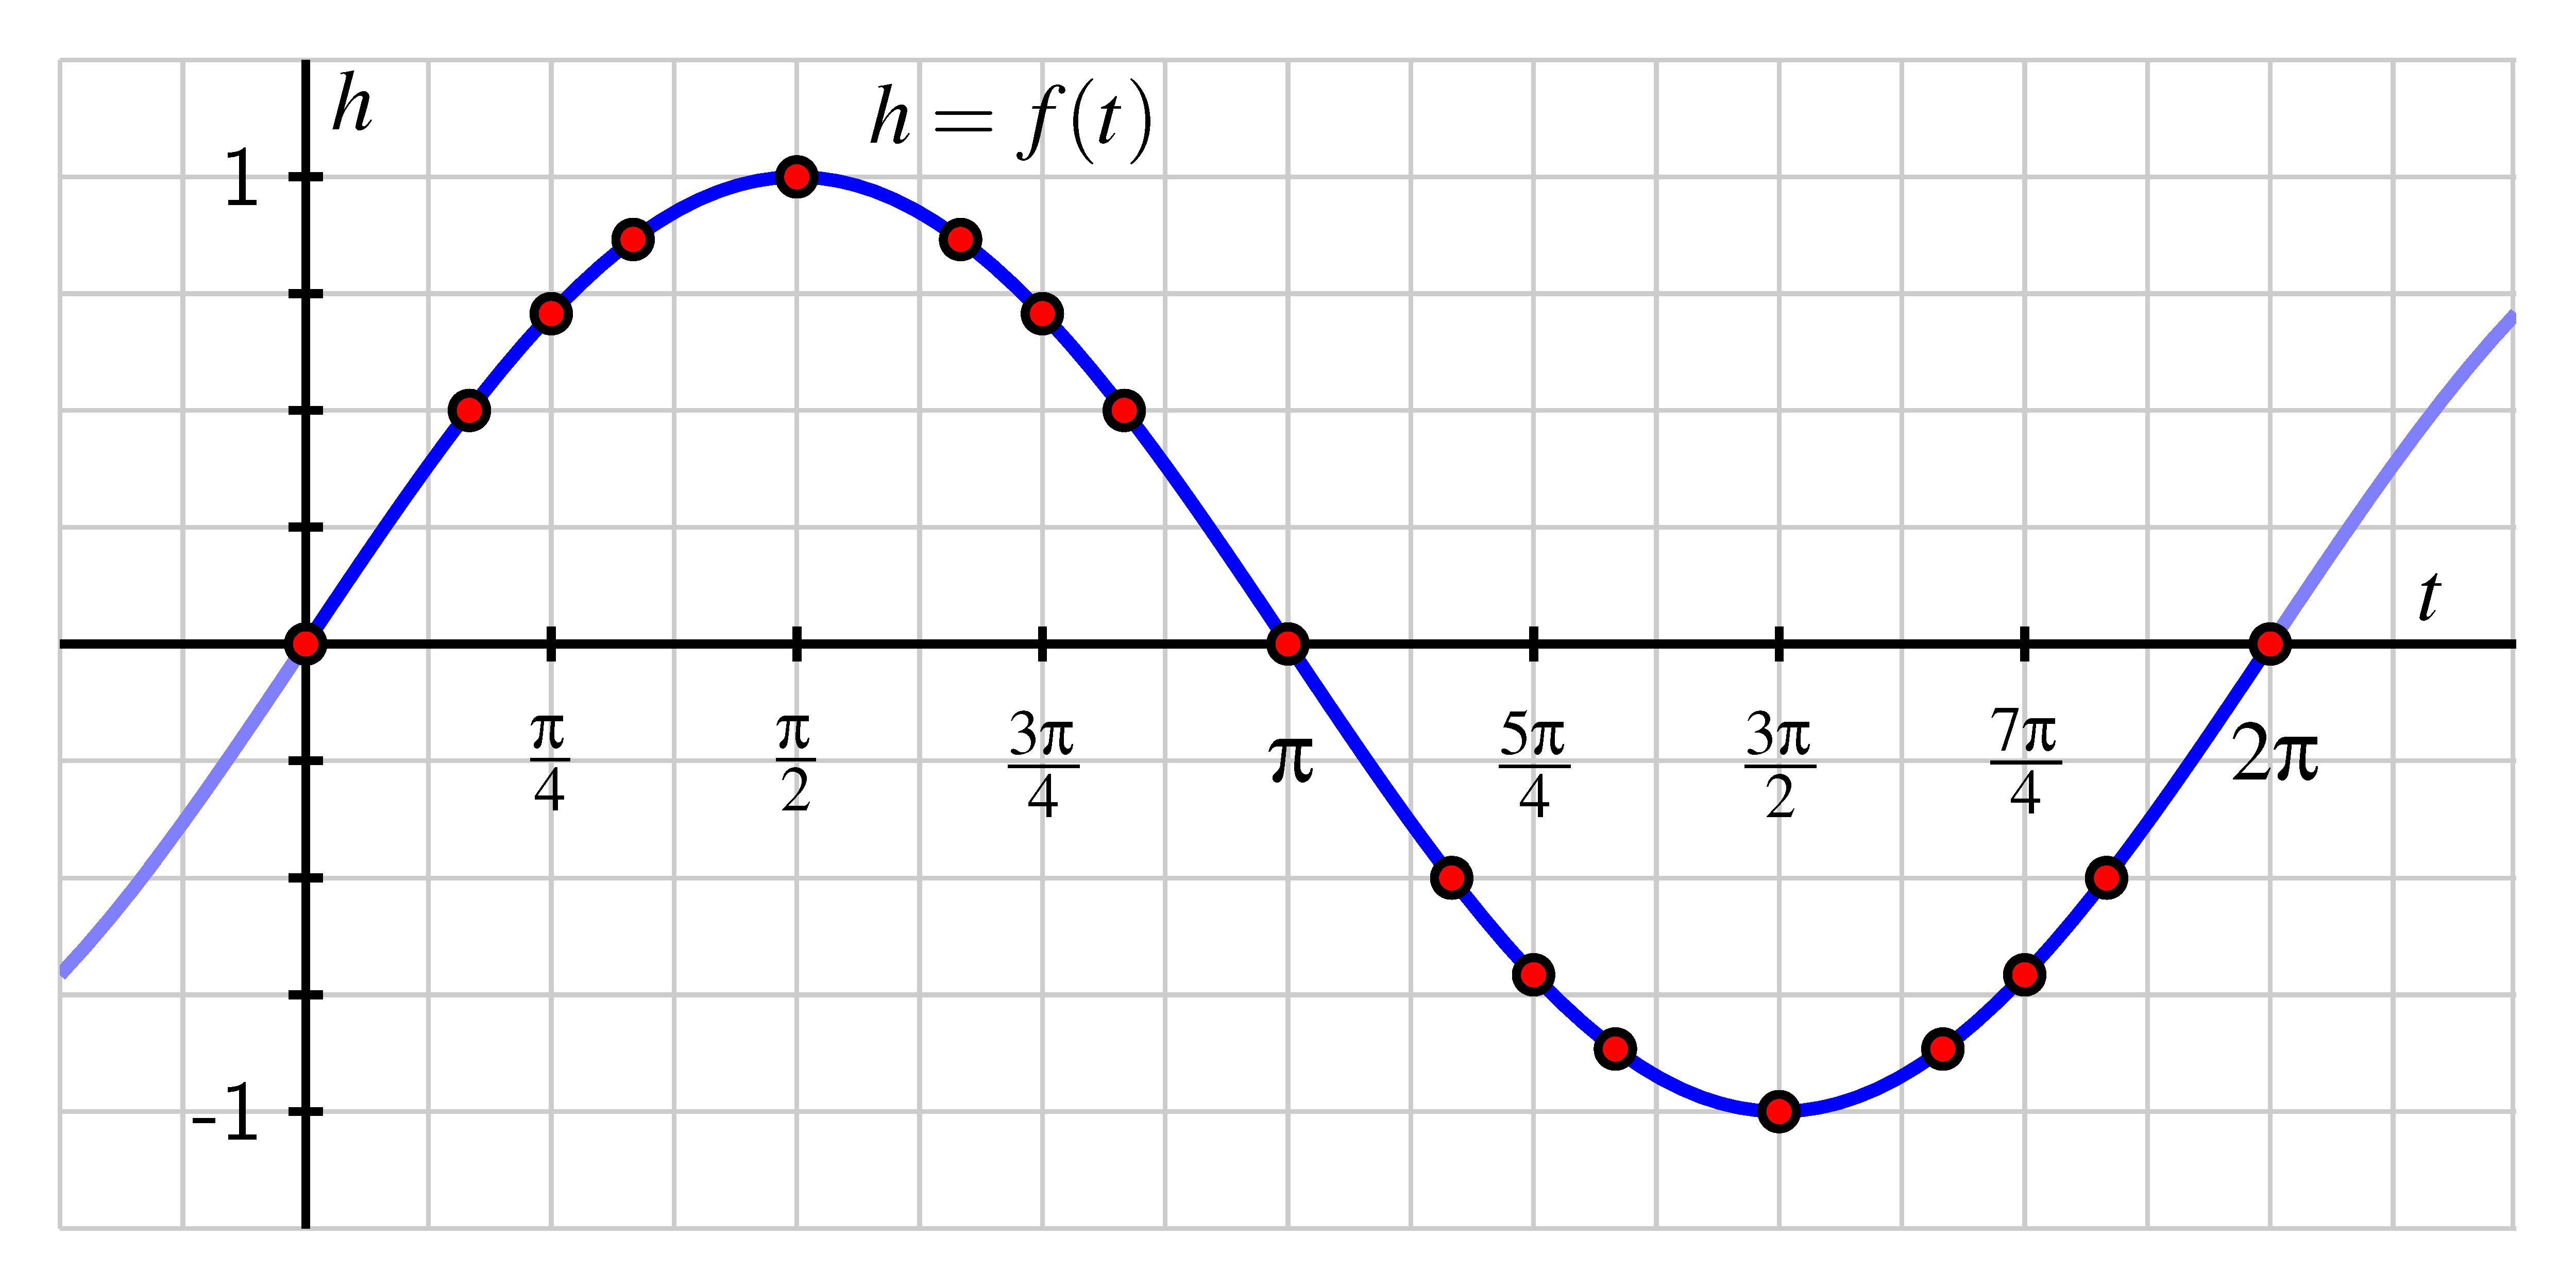
\includegraphics{sine-labeling-graph.png}
\end{image}

\begin{enumerate}[label=\alph*.]
\item
What is the exact value of \(h\left( \frac{\pi}{4} \right)\)? of \(h\left( \frac{\pi}{3} \right)\)?%
\item
Complete the following table with the exact values of \(h\) that correspond to the stated inputs.%
\[
\begin{array}{llllllllll}
t&0&\frac{\pi}{6}&\frac{\pi}{4}&\frac{\pi}{3}&\frac{\pi}{2}&\frac{2\pi}{3}&\frac{3\pi}{4}&\frac{5\pi}{6}&\pi\\
\hline
h&&&&&&&&&\\
&&&&&&&&&\\
t&\pi&\frac{7\pi}{6}&\frac{5\pi}{4}&\frac{4\pi}{3}&\frac{3\pi}{2}&\frac{5\pi}{3}&\frac{7\pi}{4}&\frac{11\pi}{6}&2\pi\\
\hline
h&&&&&&&&&
\end{array}
\]
\item
What is the exact value of \(h\left( \frac{11\pi}{4} \right)\)? of \(h\left( \frac{14\pi}{3} \right)\)?%
\item
Give four different values of \(t\) for which \(h(t) = -\frac{\sqrt{3}}{2}\).%
\end{enumerate}

\end{exploration}


%\typeout{************************************************}

\section{The Definition of the Sine Function}

The circular function that tracks the height of a point on the unit circle traversing counterclockwise from \((1,0)\) as a function of the corresponding central angle (in radians) is one of the most important functions in mathematics.  As such, we give the function a name:  the \dfn{sine} function.%

\begin{definition}
\index{sine function}
\begin{image}
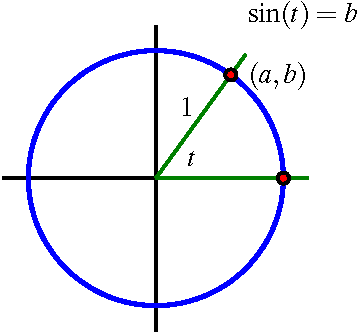
\includegraphics{sine-defn.png}
\end{image}
Given a central angle in the unit circle that measures \(t\) radians and that intersects the circle at both \((1,0)\) and \((a,b)\), we define the \dfn{sine of \(t\)}, denoted \(\sin(t)\), by the rule
\begin{equation*}
\sin(t) = b\text{.}
\end{equation*}
\end{definition}

Because of the correspondence between radian angle measure and distance traversed on the unit circle, we can also think of \(\sin(t)\) as identifying the \(y\)-coordinate of the point after it has traveled \(t\) units counterclockwise along the circle from \((1,0)\).  Note particularly that we can consider the sine of negative inputs:  for instance, \(\sin\left(-\frac{\pi}{2}\right) = -1\).

Based on our earlier work with the unit circle, we know many different exact values of the sine function, and summarize these in in the table below:
\[
\begin{array}{llllllllll}
t&0&\frac{\pi}{6}&\frac{\pi}{4}&\frac{\pi}{3}&\frac{\pi}{2}&\frac{2\pi}{3}&\frac{3\pi}{4}&\frac{5\pi}{6}&\pi\\[8pt]
\hline \\[-3ex]
%&&&&&&&&&\\
\sin(t)&0&\frac{1}{2}&\frac{\sqrt{2}}{2}&\frac{\sqrt{3}}{2}&1&\frac{\sqrt{3}}{2}&\frac{\sqrt{2}}{2}&\frac{1}{2}&0\\[10pt]
&&&&&&&&&\\
%&&&&&&&&&\\
t&\pi&\frac{7\pi}{6}&\frac{5\pi}{4}&\frac{4\pi}{3}&\frac{3\pi}{2}&\frac{5\pi}{3}&\frac{7\pi}{4}&\frac{11\pi}{6}&2\pi\\[8pt]
%&&&&&&&&&\\
\hline\\[-3ex]
%&&&&&&&&&\\
\sin(t)&0&-\frac{1}{2}&-\frac{\sqrt{2}}{2}&-\frac{\sqrt{3}}{2}&-1&-\frac{\sqrt{3}}{2}&-\frac{\sqrt{2}}{2}&-\frac{1}{2}&0
\end{array}
\]

Moreover, if we now plot these points in the usual way, we get the familiar circular wave function that comes from tracking the height of a point traversing a circle.  We often call this graph the \dfn{sine wave}.

\begin{image}
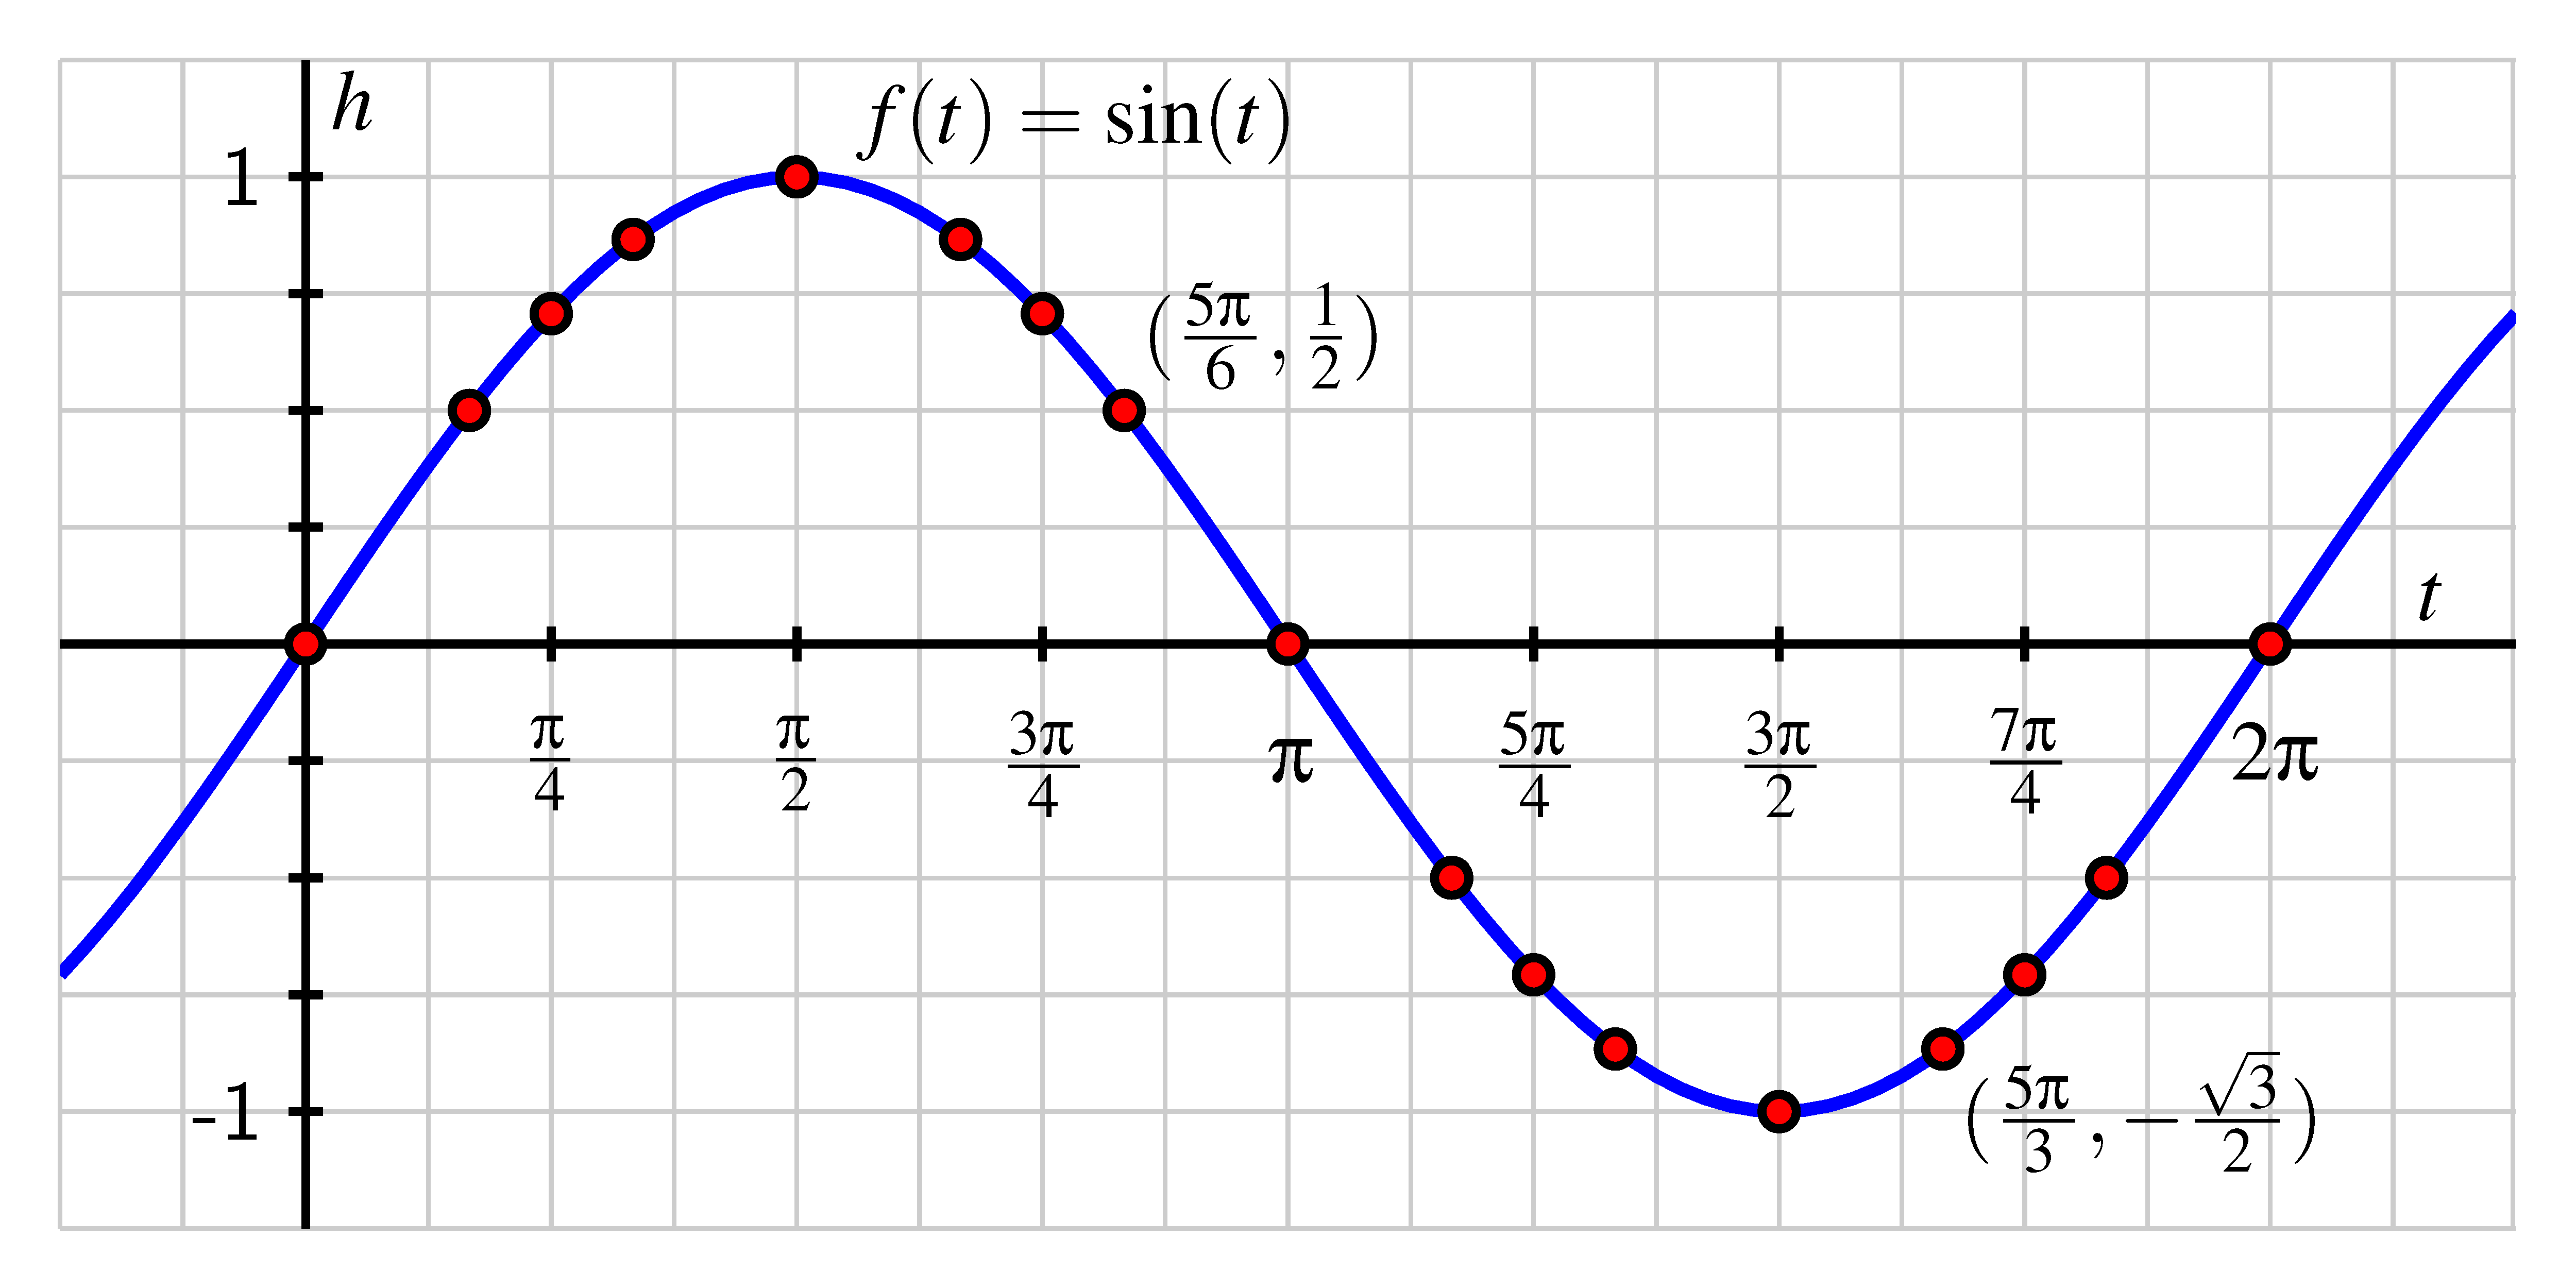
\includegraphics{sine-definition-graph.png}
\end{image}

At \link{https://www.desmos.com/calculator/f9foqx24ct} you can explore and investigate a helpful Desmos animation that shows how this motion around the circle generates the sine graph.

\begin{center}  
\desmos{f9foqx24ct}{800}{600}  
\end{center} 

%\typeout{************************************************}

\section{The Definition of the Cosine Function}

Given any central angle of radian measure \(t\) in the unit circle with one side passing through the point \((1,0)\), the angle generates a unique point \((a,b)\) that lies on the circle.  Just as we can view the \(y\)-coordinate as a function of \(t\), the \(x\)-coordinate is likewise a function of \(t\).  We therefore make the following definition.

\begin{definition}
\index{cosine function}
\begin{image}
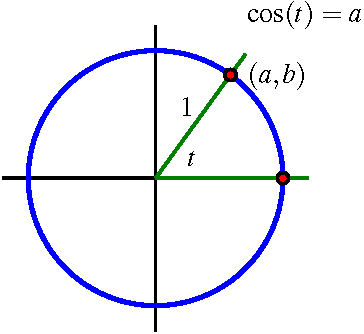
\includegraphics{sine-defn-cosine.png}
\end{image}
Given a central angle in the unit circle that measures \(t\) radians and that intersects the circle at both \((1,0)\) and \((a,b)\), we define the \dfn{cosine of \(t\)}, denoted \(\cos(t)\), by the rule
\begin{equation*}
\cos(t) = a\text{.}
\end{equation*}
\end{definition}

Again because of the correspondence between the radian measure of an angle and arc length along the unit circle, we can view the value of \(\cos(t)\) as tracking the \(x\)-coordinate of a point traversing the unit circle clockwise a distance of \(t\) units along the circle from \((1,0)\).  We now use the data and information we have developed about the unit circle to build a table of values of \(\cos(t)\) as well as a graph of the curve it generates.

\begin{exploration}
Let \(k = g(t)\) be the function that tracks the \(x\)-coordinate of a point traversing the unit circle counterclockwise from \((1,0)\).  That is, \(g(t) = \cos(t)\).  Use the information we know about the unit circle to respond to the following questions.

\begin{image}
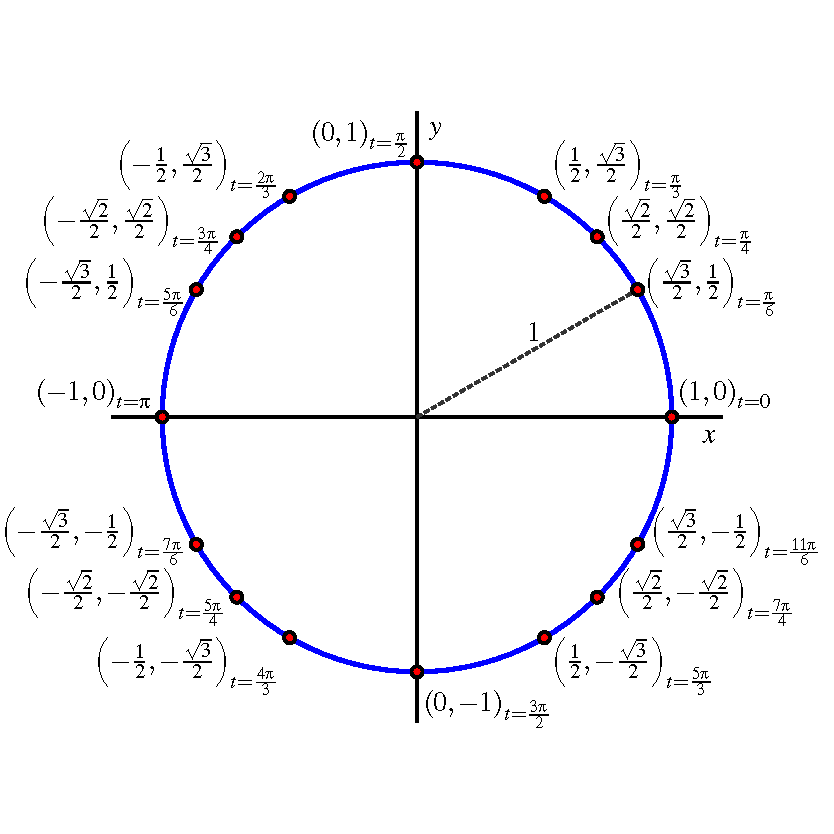
\includegraphics{unit-circle-16-all-labeled.png}
\end{image}

\begin{enumerate}[label=\alph*.]
\item What is the exact value of \(\cos\left(\frac{\pi}{6}\right)\)?  of \(\cos\left(\frac{5\pi}{6}\right)\)? \(\cos\left(-\frac{\pi}{3}\right)\)?
\item Complete the following table with the exact values of \(k\) that correspond to the stated inputs.
\[
\begin{array}{llllllllll}
t&0&\frac{\pi}{6}&\frac{\pi}{4}&\frac{\pi}{3}&\frac{\pi}{2}&\frac{2\pi}{3}&\frac{3\pi}{4}&\frac{5\pi}{6}&\pi\\
\hline
k&&&&&&&&&\\
&&&&&&&&&\\
t&\pi&\frac{7\pi}{6}&\frac{5\pi}{4}&\frac{4\pi}{3}&\frac{3\pi}{2}&\frac{5\pi}{3}&\frac{7\pi}{4}&\frac{11\pi}{6}&2\pi\\
\hline
k&&&&&&&&&
\end{array}
\]
\item On the axes provided, sketch an accurate graph of \(k = \cos(t)\).  Label the exact location of several key points on the curve.
\begin{image}
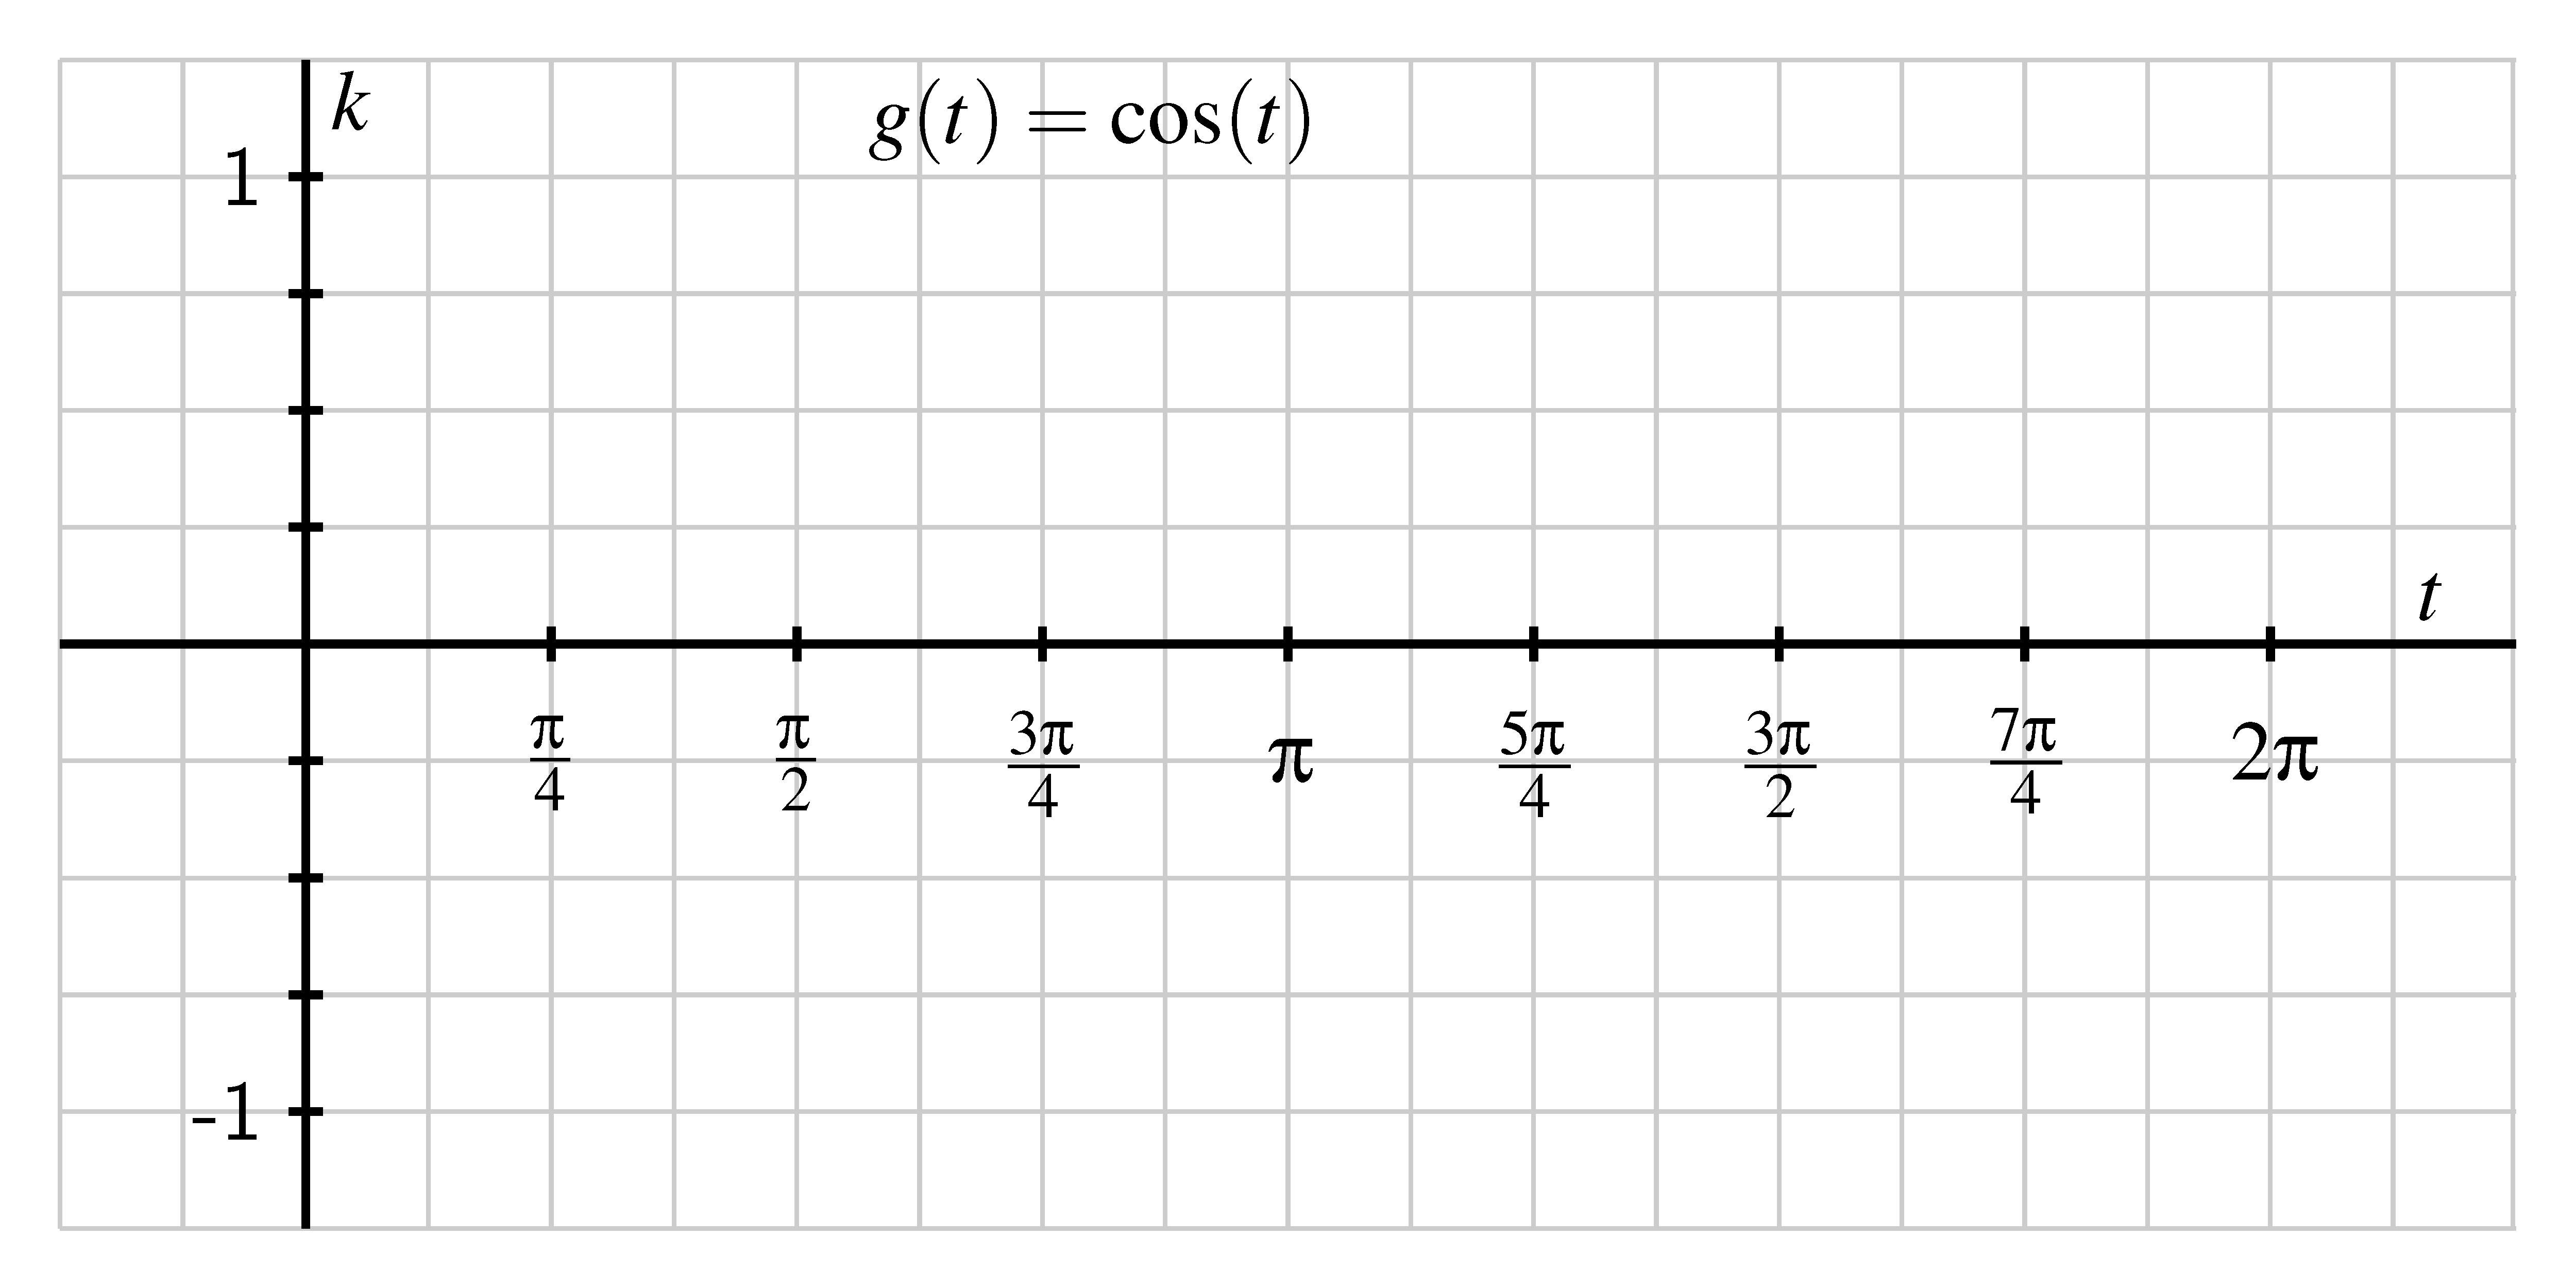
\includegraphics{sine-cosine-definition-axes.png}
\end{image}
\item What is the exact value of \(\cos\left( \frac{11\pi}{4} \right)\)? of \(\cos\left( \frac{14\pi}{3} \right)\)?
\item Give four different values of \(t\) for which \(\cos(t) = -\frac{\sqrt{3}}{2}\).
\item How is the graph of \(k = \cos(t)\) different from the graph of \(h = \sin(t)\)?  How are the graphs similar?
\end{enumerate}

\end{exploration}

As we work with the sine and cosine functions, it's always helpful to remember their definitions in terms of the unit circle and the motion of a point traversing the circle.  At \link{https://www.desmos.com/calculator/9s1ms0nlyf} you can explore and investigate a helpful Desmos animation that shows how this motion around the circle generates the cosine graph.

\begin{center}  
\desmos{9s1ms0nlyf}{800}{600}  
\end{center} 

%\typeout{************************************************}

\section{Properties of Sine and Cosine}
Because the sine function results from tracking the \(y\)-coordinate of a point traversing the unit circle and the cosine function from the \(x\)-coordinate, the two functions have several shared properties of circular functions.

\begin{callout}
For both \(f(t) = \sin(t)\) and \(g(t) = \cos(t)\),%
\begin{itemize}[label=\textbullet]
\item
the domain of the function is all real numbers;%
\item
the range of the function is \([-1,1]\);%
\item
the midline of the function is \(y = 0\);%
\item
the amplitude of the function is \(a = 1\);%
\item
the period of the function is \(p = 2\pi\).%
\end{itemize}
\end{callout}

It is also insightful to juxtapose the sine and cosine functions' graphs on the same coordinate axes.  When we do, as seen in the figure below%\hyperref[F-sine-cosine-both]{Figure~\ref{F-sine-cosine-both}}
, we see that the curves can be viewed as horizontal translations of one another.%

\begin{image}
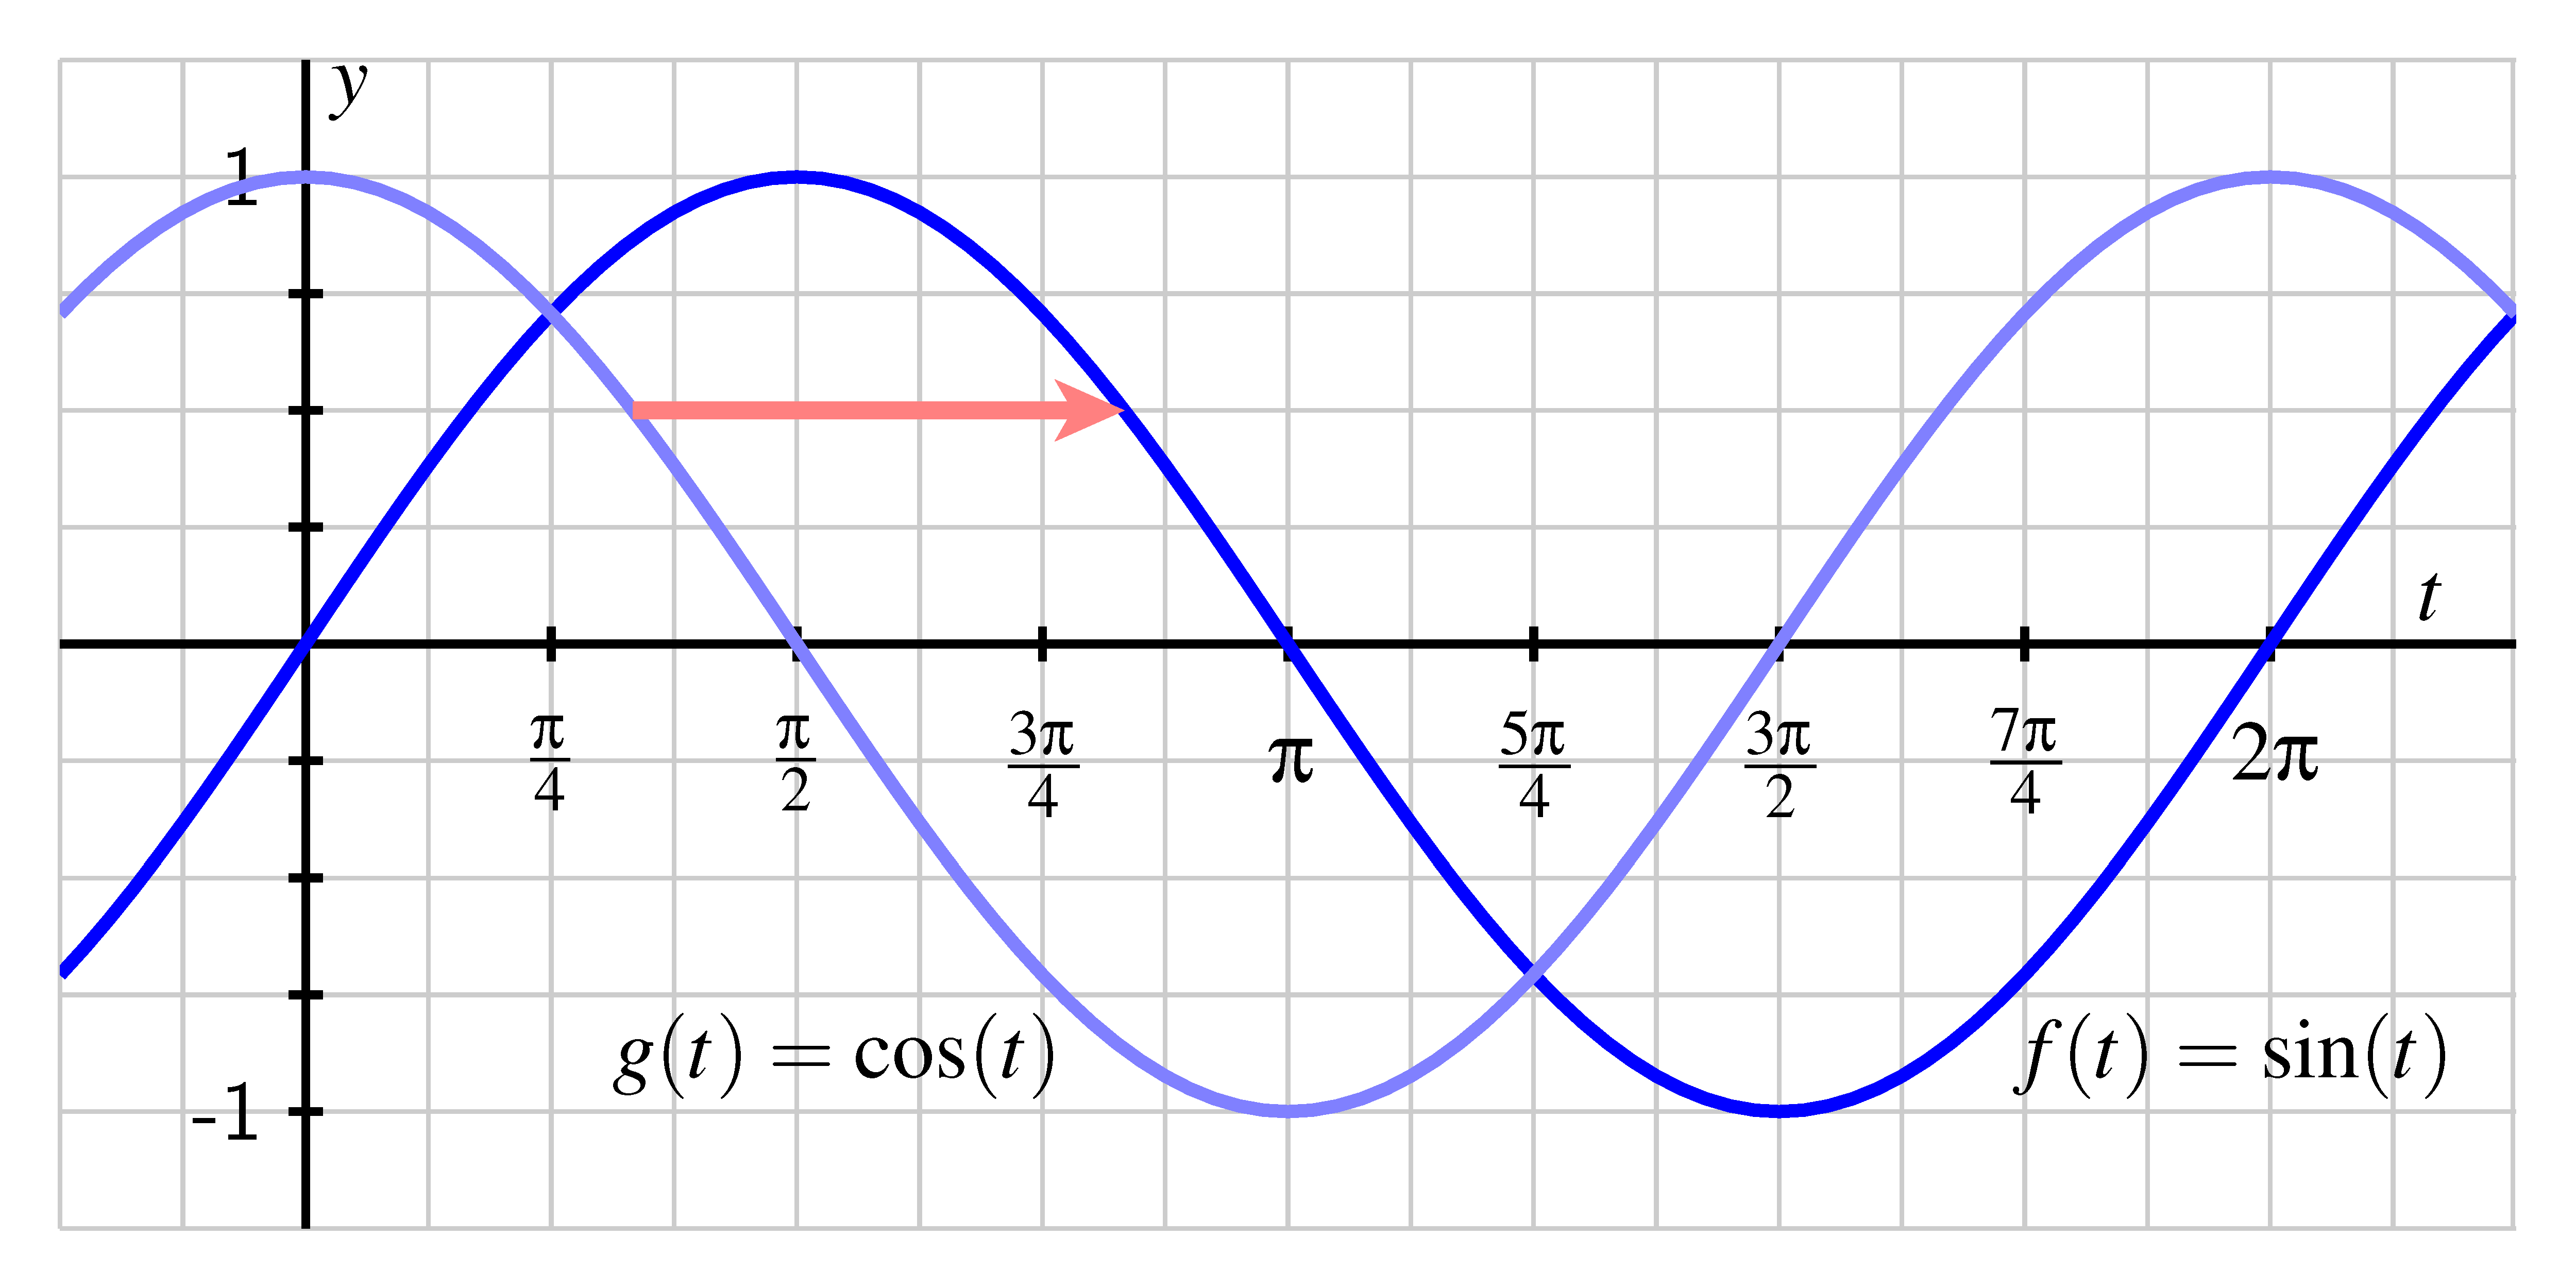
\includegraphics{sine-and-cosine-graphs.png}
\end{image}

In particular, since the sine graph can be viewed as the cosine graph shifted \(\frac{\pi}{2}\) units to the right, it follows that for any value of \(t\),%
\begin{equation*}
\sin(t) = \cos\left(t-\frac{\pi}{2}\right)\text{.}
\end{equation*}
Similarly, since the cosine graph can be viewed as the sine graph shifted left,%
\begin{equation*}
\cos(t) = \sin\left(t + \frac{\pi}{2}\right)\text{.}
\end{equation*}
Because each of the two preceding equations hold for every value of \(t\), they are often referred to as \emph{identities}.%
\par
\hypertarget{p-1054}{}%
In light of the definitions of the sine and cosine functions, we can now view any point \((x,y)\) on the unit circle as being of the form \((\cos(t),\sin(t))\), where \(t\) is the measure of the angle whose vertices are \((1,0)\), \((0,0)\), and \((x,y)\).  Note particularly that since \(x^2 + y^2 = 1\), it is also true that \(\cos^2(t) + \sin^2(t) = 1\).  We call this fact the Fundamental Trigonometric Identity.%

\begin{callout}
For any real number \(t\),%
\begin{equation*}
\cos^2(t) + \sin^2(t) = 1\text{.}
\end{equation*}
\end{callout}

There are additional trends and patterns in the two functions' graphs that we explore further in the following activity.

\begin{exploration}
Use the figure below to assist in answering the following questions.
\begin{image}
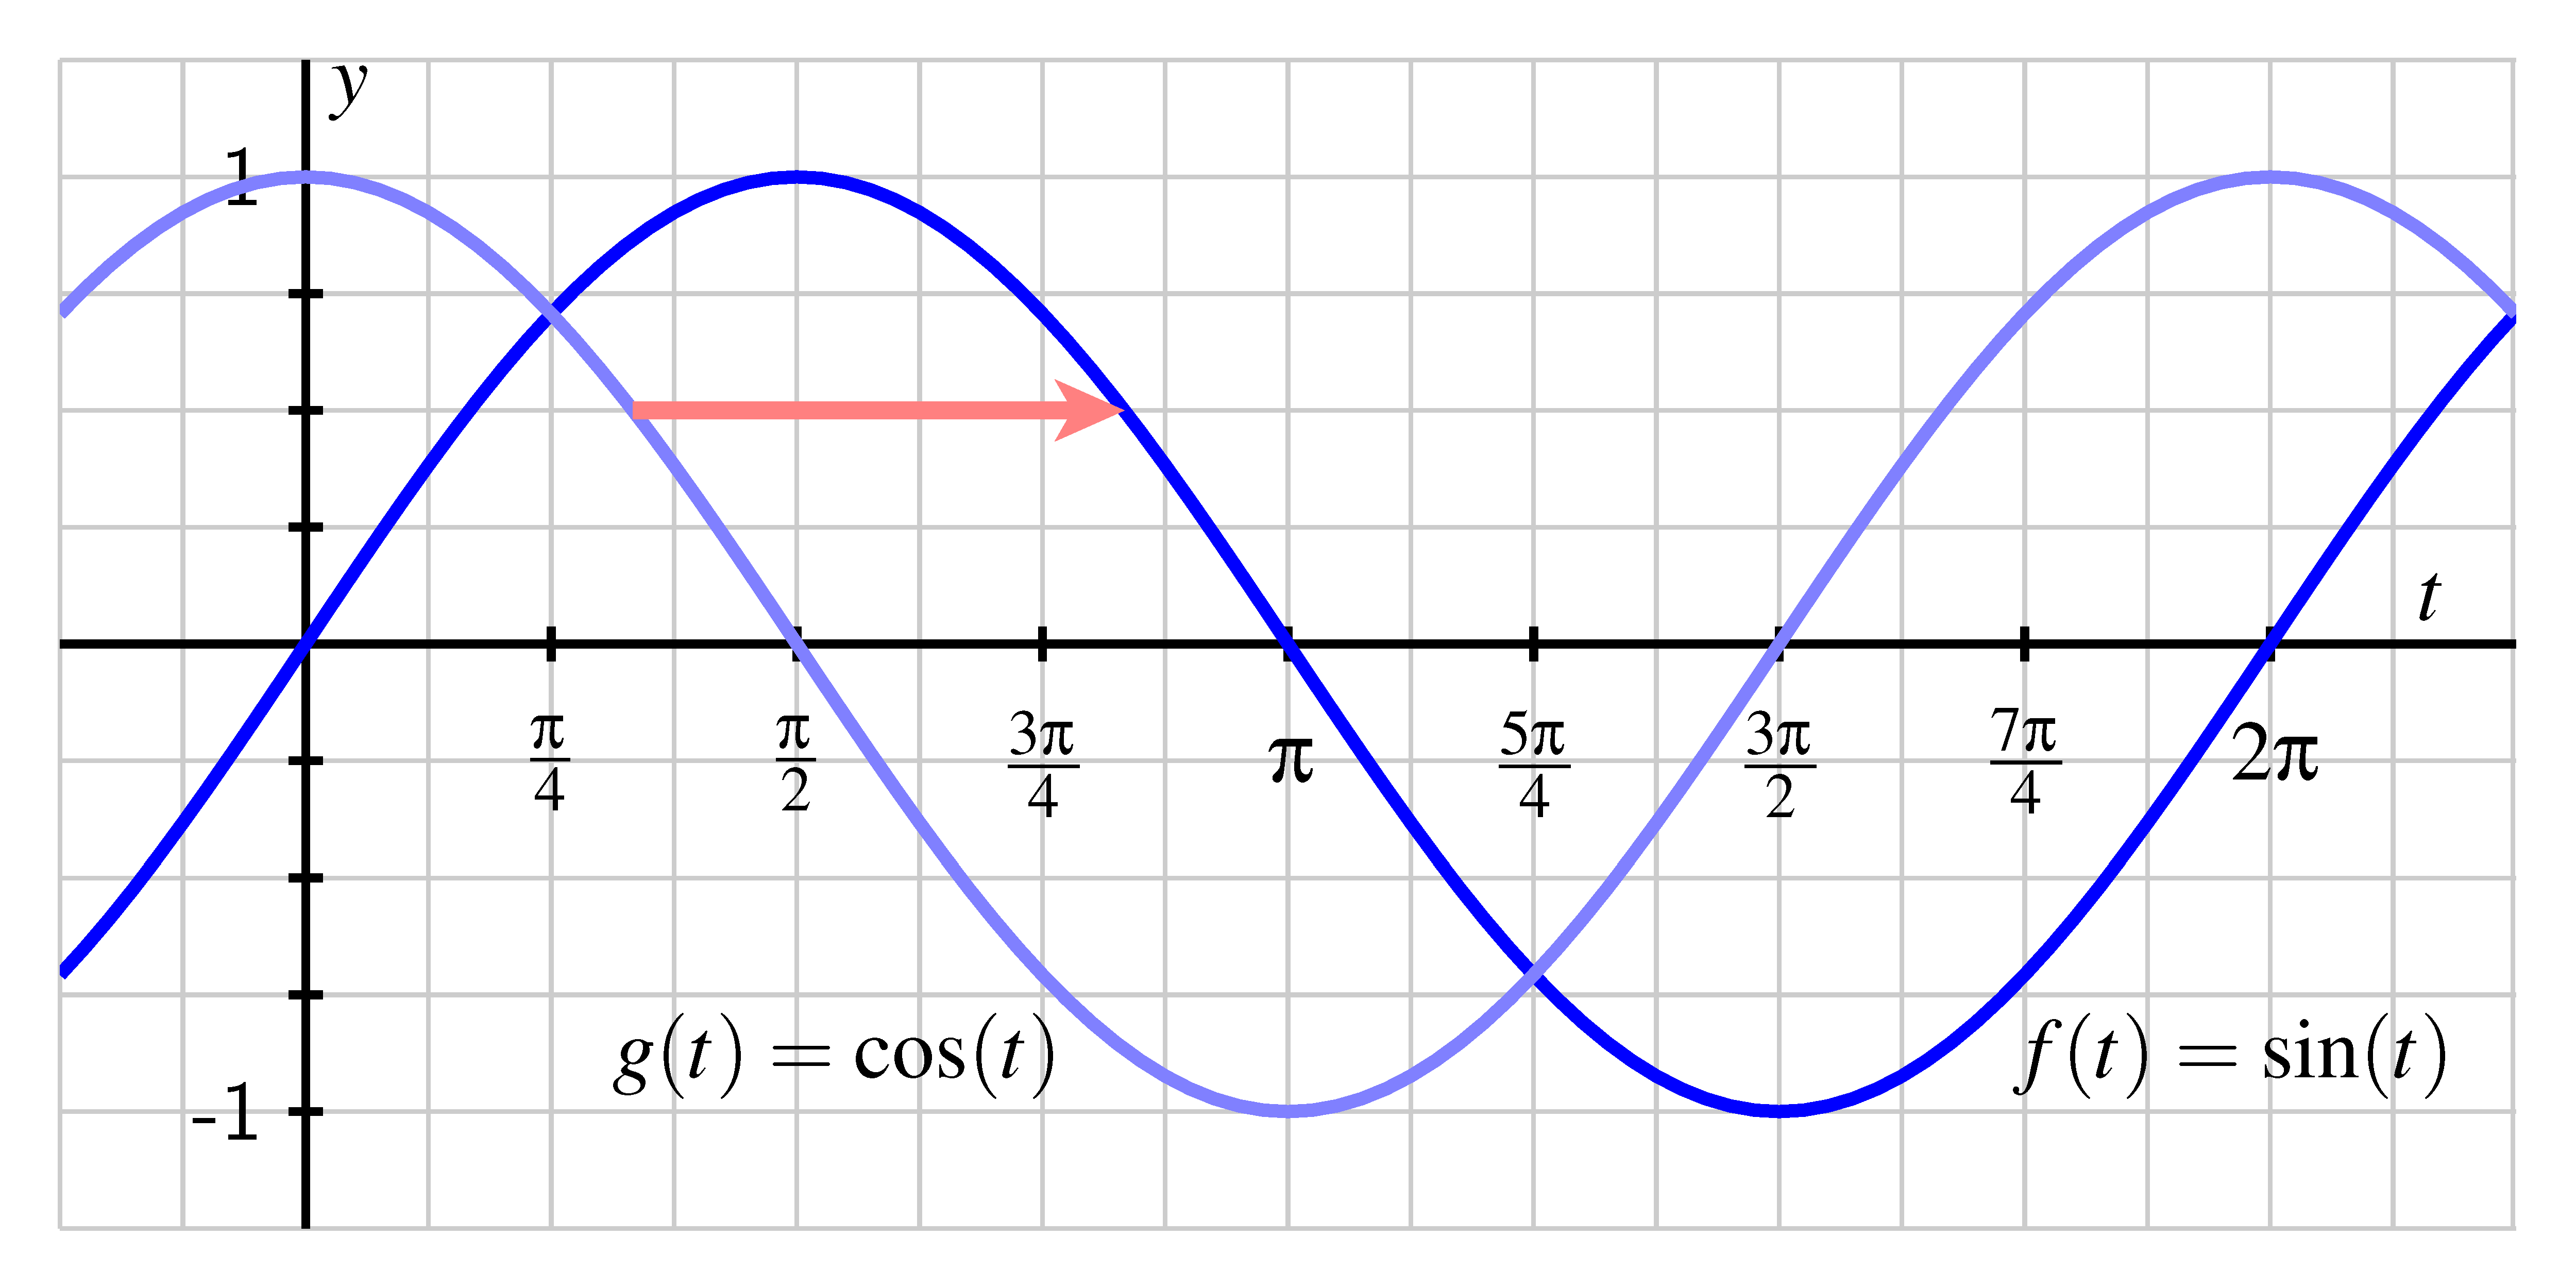
\includegraphics{sine-and-cosine-graphs.png}
\end{image}

\begin{enumerate}[label=\alph*.]
\item
Give an example of the largest interval you can find on which \(f(t) = \sin(t)\) is decreasing.%
\item
Give an example of the largest interval you can find on which \(f(t) = \sin(t)\) is decreasing and concave down.%
\item
Give an example of the largest interval you can find on which \(g(t) = \cos(t)\) is increasing.%
\item
Give an example of the largest interval you can find on which \(g(t) = \sin(t)\) is increasing and concave up.%
\item
Without doing any computation, on which interval is the average rate of change of \(g(t) = \cos(t)\) greater:  \(\left[\pi, \pi+0.1\right]\) or \(\left[\frac{3\pi}{2}, \frac{3\pi}{2} + 0.1\right]\)?  Why?%
\item
In general, how would you characterize the locations on the sine and cosine graphs where the functions are increasing or decreasingly most rapidly?%
\item
For which quadrants of the \(x\)-\(y\) plane is \(\cos(t)\) negative for an angle in that quadrant?%
\end{enumerate}

\end{exploration}

%\typeout{************************************************}

\section{Using Computing Technology}

We have established that we know the exact value of \(\sin(t)\) and \(\cos(t)\) for any of the \(t\)-values labeled on the unit circle, as well as for any such \(t \pm 2j\pi\), where \(j\) is a whole number, due to the periodicity of the functions.  But what if we want to know \(\sin(1.35)\) or \(\cos\left(\frac{\pi}{5}\right)\) or values for other inputs not in the table?%

Any standard computing device a scientific calculator, \emph{Desmos}, \emph{Geogebra}, \emph{WolframAlpha}, etc. has the ability to evaluate the sine and cosine functions at any input we desire.  Because the input is viewed as an angle, each computing device has the option to consider the angle in radians or degrees.  \emph{It is always essential that you are sure which type of input your device is expecting.}  Our computational device of choice is \emph{Desmos}.  In \emph{Desmos}, you can change the input type between radians and degrees by clicking the wrench icon in the upper right and choosing the desired units.  Radians is the default, and radians is what we will primarily use in both this class and calculus.%

It take substantial and sophisticated mathematics to enable a computational device to evaluate the sine and cosine functions at any value we want; the algorithms involve an idea from calculus known as an infinite series.  While your computational device is powerful, it's both helpful and important to understand the meaning of these values on the unit circle and to remember the special points for which we know the outputs of the sine and cosine functions exactly.%
\begin{exploration}

Answer the following questions exactly wherever possible.  If you estimate a value, do so to at least \(5\) decimal places of accuracy.%

\begin{enumerate}[label=\alph*.]
\item
The \(x\) coordinate of the point on the unit circle that lies in the third quadrant and whose \(y\)-coordinate is \(y = -\frac{3}{4}\).%
\item
The \(y\)-coordinate of the point on the unit circle generated by a central angle in standard position that measures \(t = 2\) radians.%
\item
The \(x\)-coordinate of the point on the unit circle generated by a central angle in standard position that measures \(t = -3.05\) radians.%
\item
The value of \(\cos(t)\) where \(t\) is an angle in Quadrant II that satisfies \(\sin(t) = \frac{1}{2}\).%
\item
The value of \(\sin(t)\) where \(t\) is an angle in Quadrant III for which \(\cos(t) = -0.7\).%
\item
The average rate of change of \(f(t) = \sin(t)\) on the intervals \([0.1,0.2]\) and \([0.8,0.9]\).%
\item
The average rate of change of \(g(t) = \cos(t)\) on the intervals \([0.1,0.2]\) and \([0.8,0.9]\).%
\end{enumerate}
%
\end{exploration}

%\typeout{************************************************}

\begin{summary}
\begin{itemize}[label=\textbullet]
\item
The sine and cosine functions result from tracking the \(y\)- and \(x\)-coordinates of a point traversing the unit circle counterclockwise from \((1,0)\).  The value of \(\sin(t)\) is the \(y\)-coordinate of a point that has traversed \(t\) units along the circle from \((1,0)\) (or equivalently that corresponds to an angle of \(t\) radians), while the value of \(\cos(t)\) is the \(x\)-coordinate of the same point.%
\item
The sine and cosine functions are both periodic functions that share the same domain (the set of all real numbers), range (the interval \([-1,1]\)), midline (\(y = 0\)), amplitude (\(a = 1\)), and period (\(P = 2\pi\)).  In addition, the sine function is horizontal shift of the cosine function by \(\frac{\pi}{2}\) units to the right, so \(\sin(t) = \cos\left(t-\frac{\pi}{2}\right)\) for any value of \(t\).%
\item
If \(t\) corresponds to one of the special angles that we know on the unit circle, we can compute the values of \(\sin(t)\) and \(\cos(t)\) exactly.  For other values of \(t\), we can use a computational device to estimate the value of either function at a given input; when we do so, we must take care to know whether we are computing in terms of radians or degrees.%
\end{itemize}
\end{summary}

\end{document}


